\documentclass{beamer}
\usepackage{tikz}
\usepackage[all]{xy}
\usepackage{amsmath,amssymb}
\usepackage{hyperref}
\usepackage{graphicx}
\usepackage{algorithmic}
\usepackage{multirow}

\DeclareMathOperator*{\argmin}{arg\,min}
\DeclareMathOperator*{\Lik}{Lik}
\DeclareMathOperator*{\PoissonLoss}{PoissonLoss}
\DeclareMathOperator*{\Peaks}{Peaks}
\DeclareMathOperator*{\Segments}{Segments}
\DeclareMathOperator*{\argmax}{arg\,max}
\DeclareMathOperator*{\maximize}{maximize}
\DeclareMathOperator*{\minimize}{minimize}
\newcommand{\sign}{\operatorname{sign}}
\newcommand{\RR}{\mathbb R}
\newcommand{\ZZ}{\mathbb Z}
\newcommand{\NN}{\mathbb N}
\newcommand{\z}{$z = 2, 4, 3, 5, 1$} 

\newcommand{\algo}[1]{\textcolor{#1}{#1}}
\definecolor{PDPA}{HTML}{66C2A5}
\definecolor{CDPA}{HTML}{FC8D62}
\definecolor{GPDPA}{HTML}{4D4D4D}

% Set transparency of non-highlighted sections in the table of
% contents slide.
\setbeamertemplate{section in toc shaded}[default][100]
\AtBeginSection[]
{
  \setbeamercolor{section in toc}{fg=red} 
  \setbeamercolor{section in toc shaded}{fg=black} 
  \begin{frame}
    \tableofcontents[currentsection]
  \end{frame}
}

\begin{document}

\title{Optimizing ROC Curves with a Sort-Based Surrogate Loss for Binary Classification and Changepoint Detection}

\author{
  Toby Dylan Hocking --- toby.hocking@nau.edu\\ 
  joint work with my student Jonathan Hillman\\
  Machine Learning Research Lab --- \url{http://ml.nau.edu}\\
  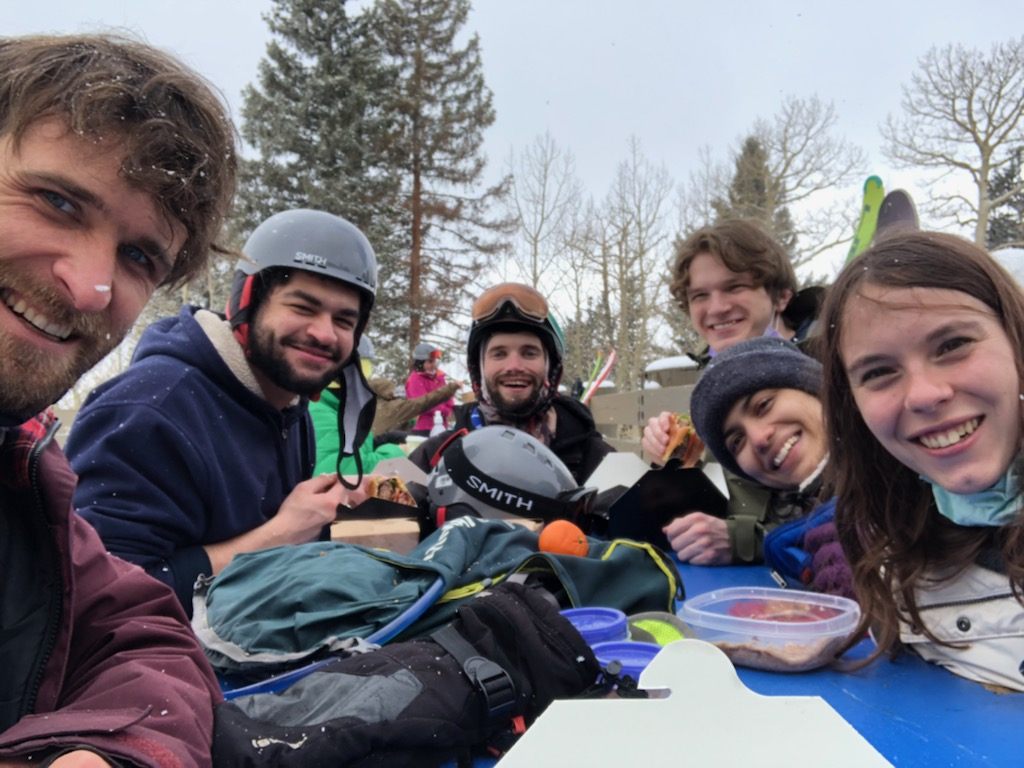
\includegraphics[height=3.5cm]{2021-03-lab-ski-lunch} \\
  Come to SICCS! Graduate Research Assistantships available!
}

\date{}

\maketitle 

\section{Problem Setting and Related Work}

\section{Results}

\begin{frame}
  \frametitle{Real data example with non-monotonic label error}

  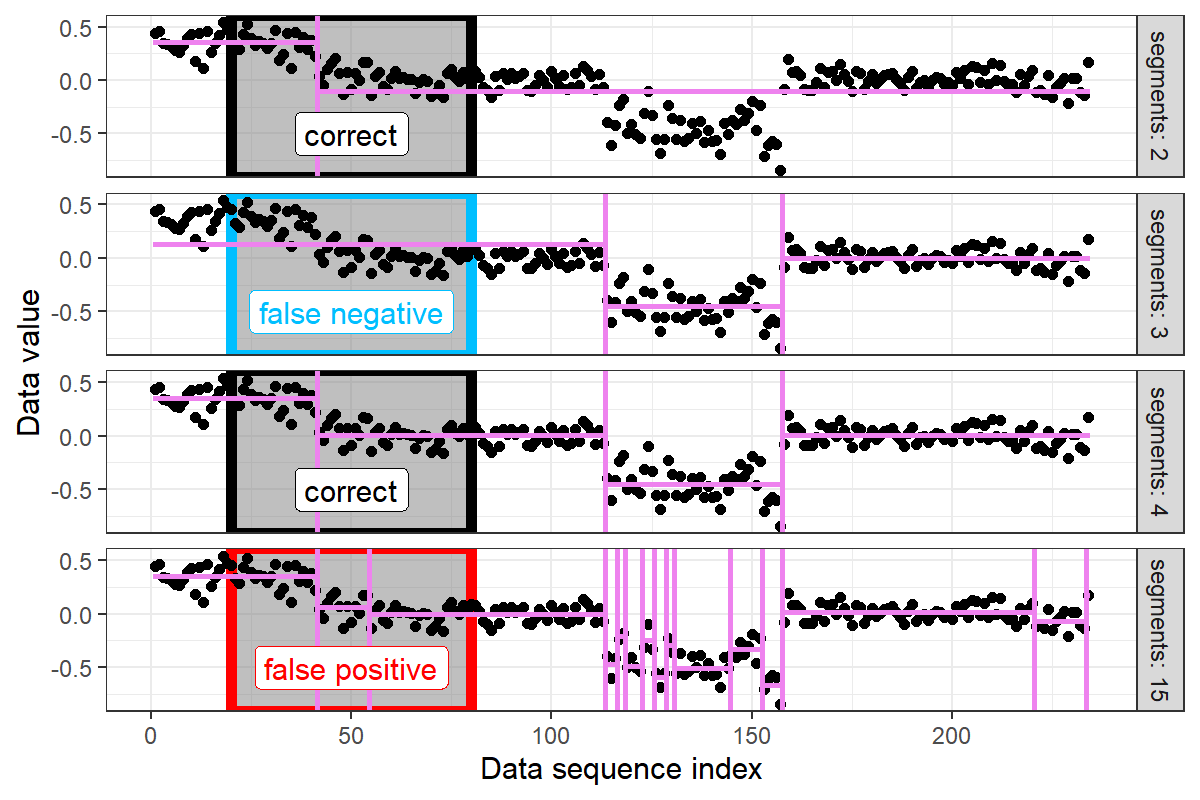
\includegraphics[width=0.49\textwidth]{figure-fn-not-monotonic}
  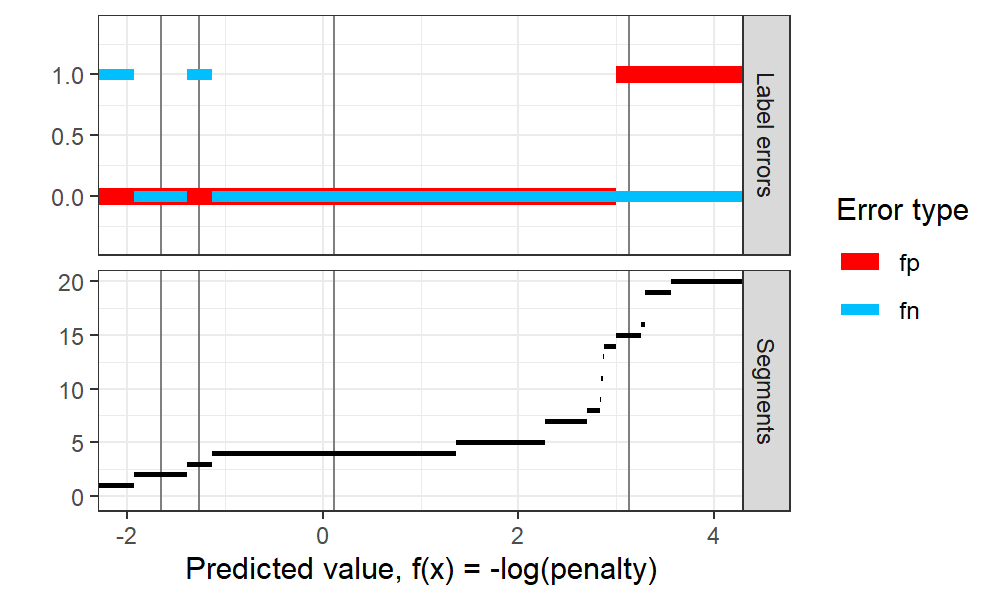
\includegraphics[width=0.49\textwidth]{figure-fn-not-monotonic-error}

\end{frame}

\begin{frame}
  \frametitle{Looping ROC curve, simple synthetic example}
  
  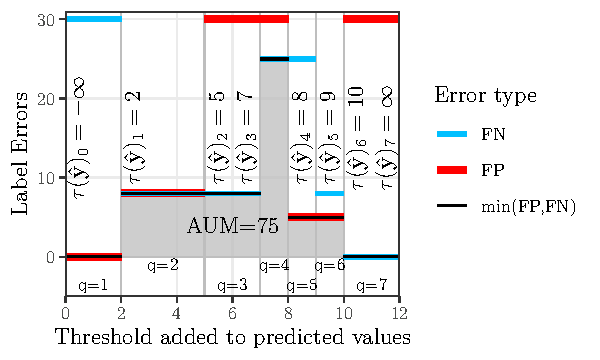
\includegraphics[height=1.5in]{figure-more-than-one-more-aum}
  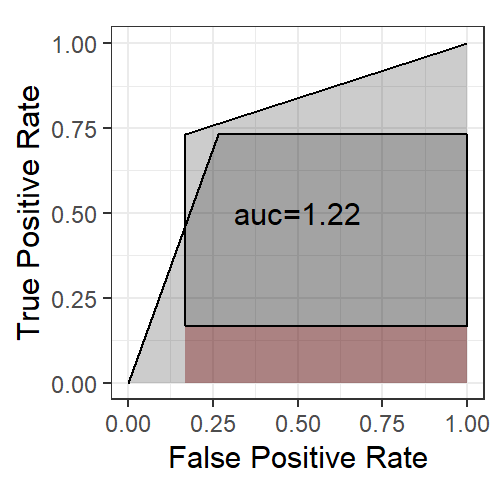
\includegraphics[height=1.5in]{figure-more-than-one-more-auc}

\end{frame}

\begin{frame}
  \frametitle{Real data example with AUC greater than one}
  
  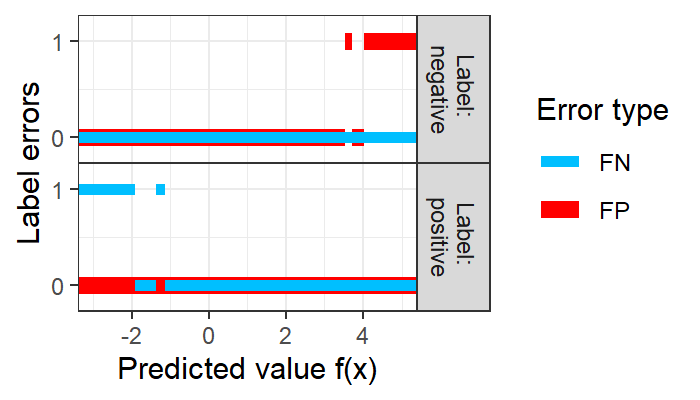
\includegraphics[height=1.3in]{figure-aum-convexity-profiles}
  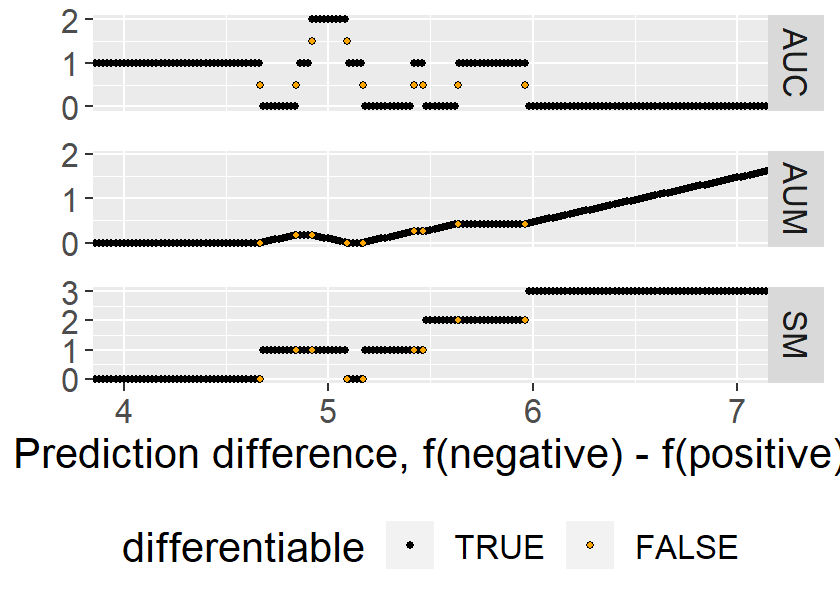
\includegraphics[height=1.3in]{figure-aum-convexity}

\end{frame}

\begin{frame}
  \frametitle{Train set ROC curves for a real changepoint problem}

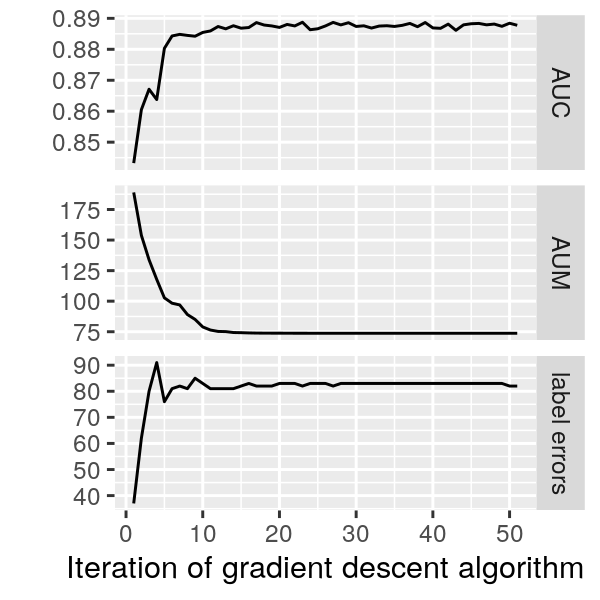
\includegraphics[height=3.7cm]{figure-aum-optimized-iterations.png}
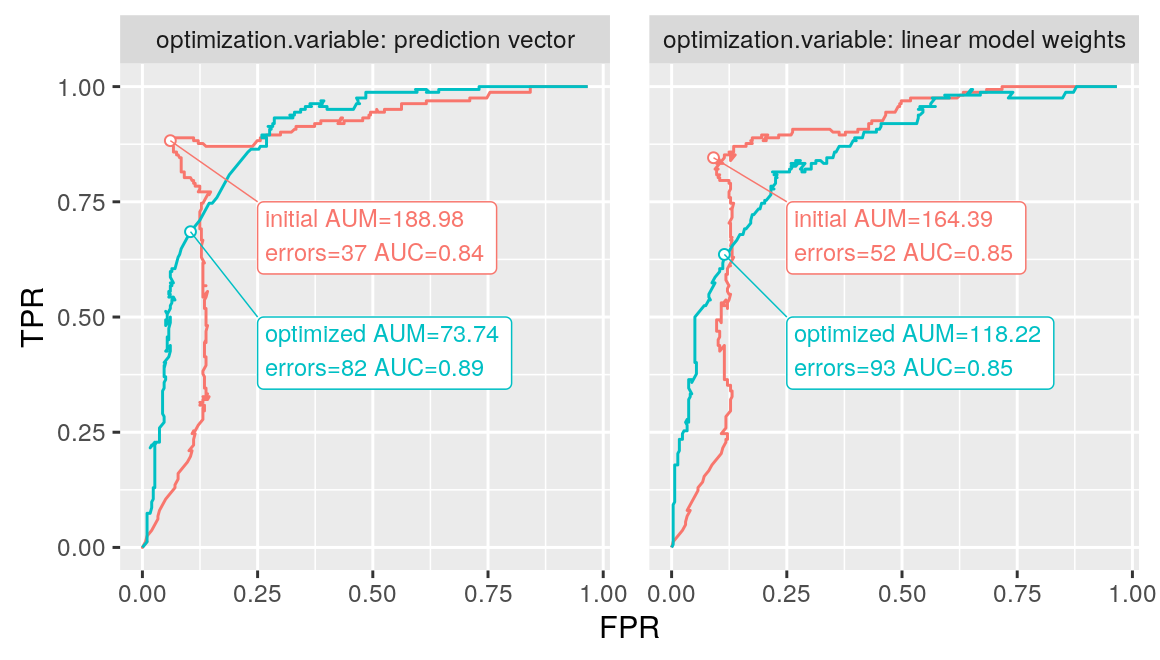
\includegraphics[height=3.7cm]{figure-aum-train-both.png}

\end{frame}

\begin{frame}
  \frametitle{Learning algorithm results in better test AUC/AUM for changepoint problems}
    
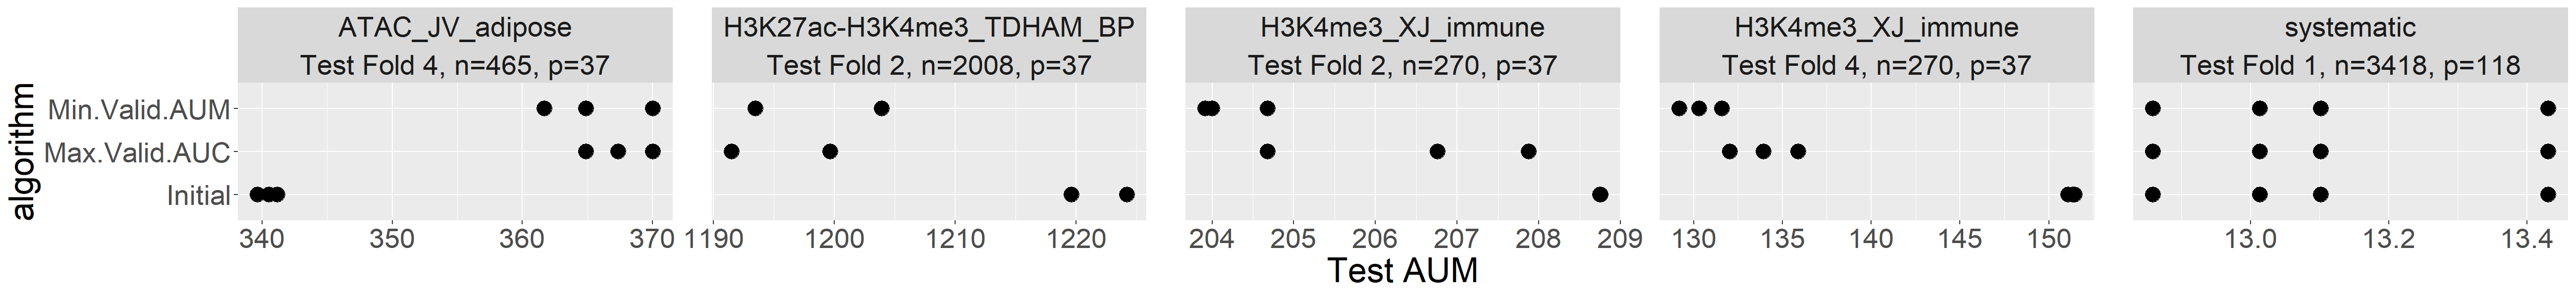
\includegraphics[width=\textwidth]{figure-test-aum-comparison.png}
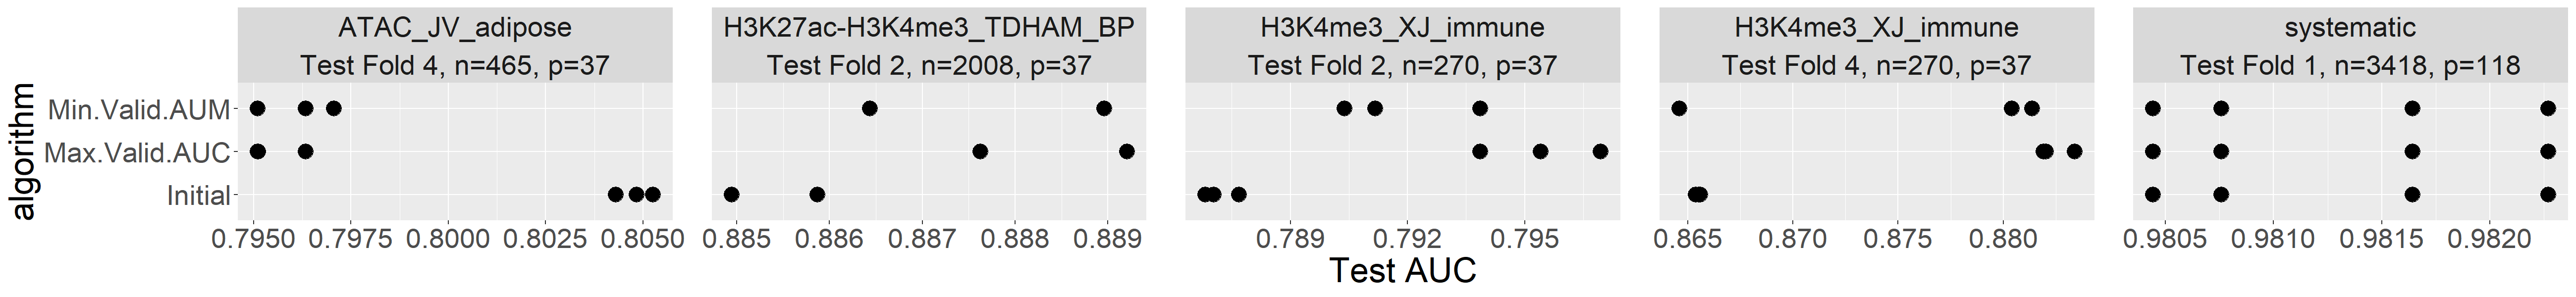
\includegraphics[width=\textwidth]{figure-test-auc-comparison.png}

\end{frame}

\begin{frame}
  \frametitle{Standard logistic loss fails for highly imbalanced labels}

 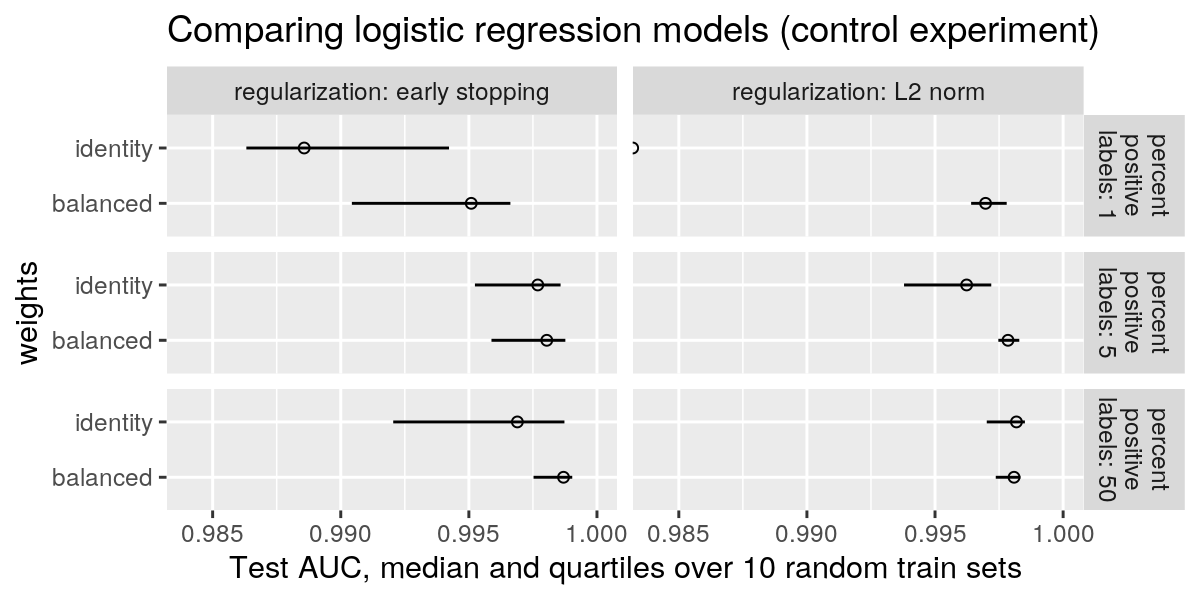
\includegraphics[width=\textwidth]{figure-unbalanced-grad-desc-logistic.png}

\end{frame}


\begin{frame}
  \frametitle{Error rate loss is not as useful as error count loss}

 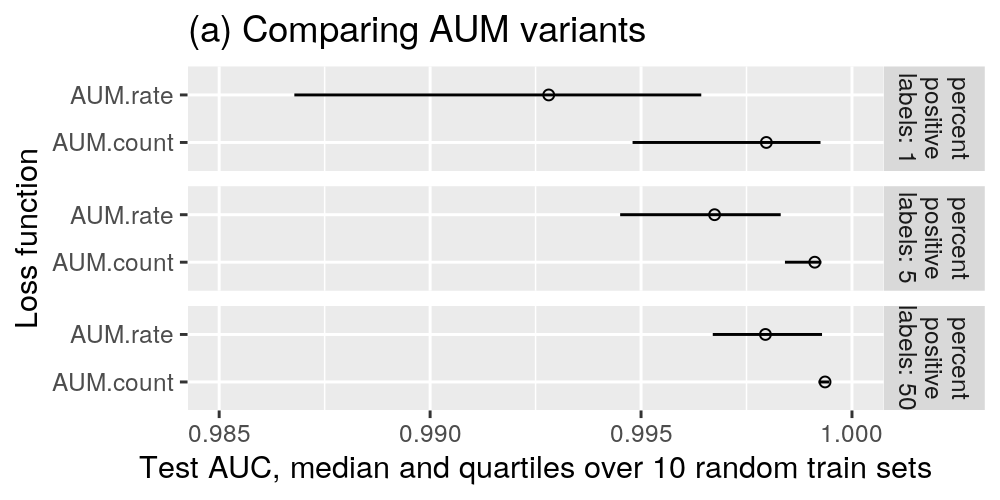
\includegraphics[width=\textwidth]{figure-unbalanced-grad-desc-aum.png}

\end{frame}

\begin{frame}
  \frametitle{Learning algorithm competitive for unbalanced binary classification}

 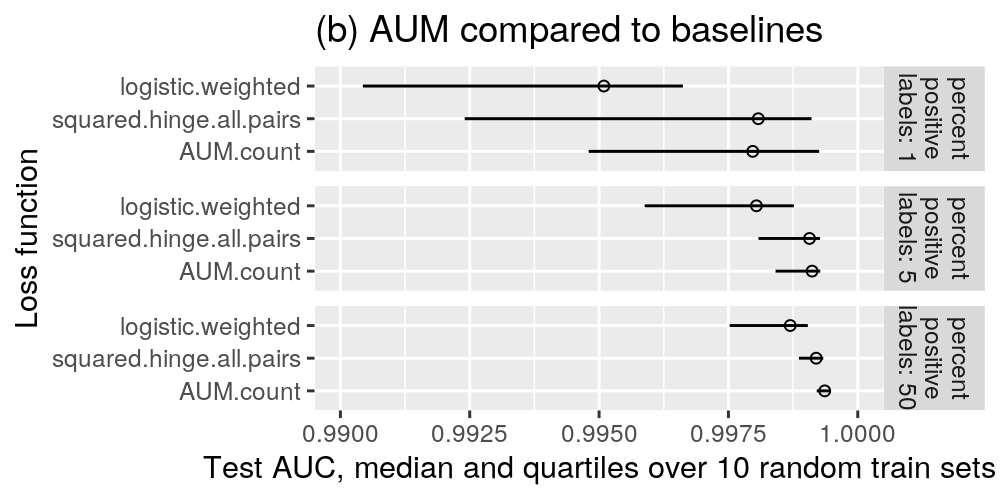
\includegraphics[width=\textwidth]{figure-unbalanced-grad-desc.png}

\end{frame}

\begin{frame}
  \frametitle{Comparable computation time to other loss functions}

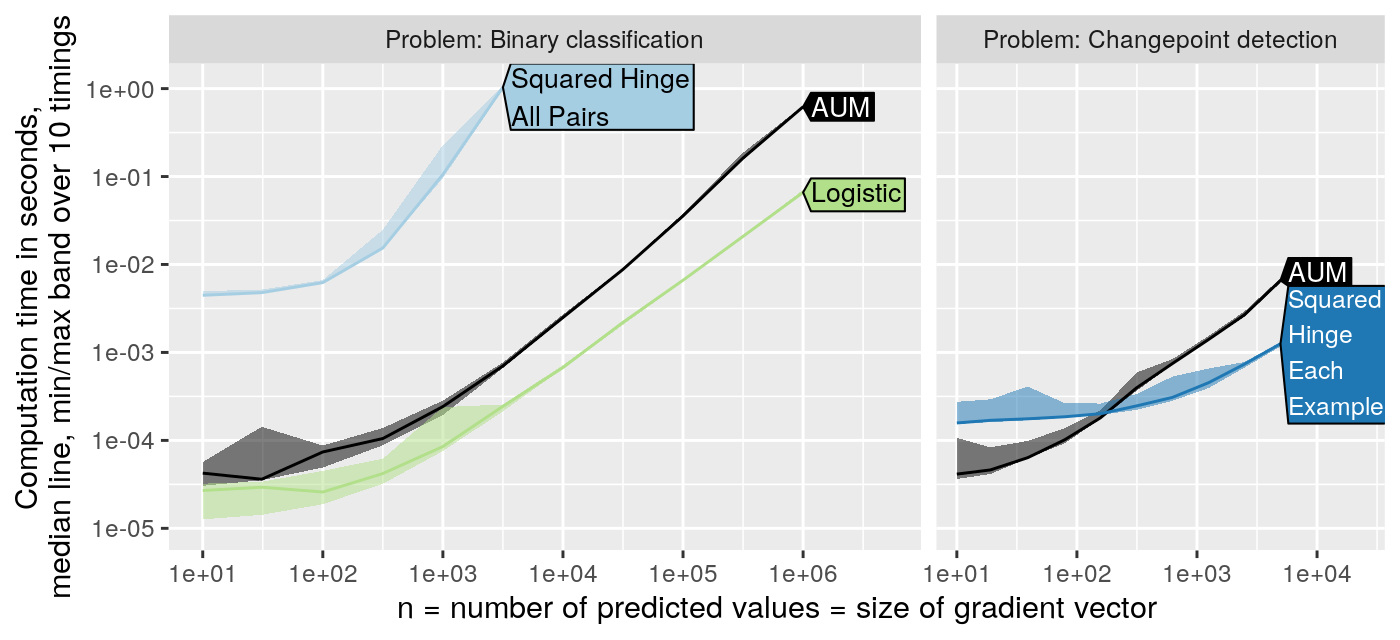
\includegraphics[width=\textwidth]{figure-aum-grad-speed-both.png}
  
\end{frame}

\end{document}
